\chapter{Epílogo: El capítulo de los senderos que se bifurcan}
\labch{epilogo}

\begin{ideanote}
El curso termina aquí, pero la estadística no. A lo largo de estas páginas abrimos muchas puertas y cruzamos sólo algunas. Este epílogo es un paseo por las que dejamos entreabiertas: temas que rozamos de pasada y que vale la pena explorar después.
\end{ideanote}

Con la regresión cerramos la materia. Pero si miramos para atrás, casi cada capítulo dejó algo pendiente: una pregunta que respondimos a medias, un \enquote{esto se puede generalizar} que no generalizamos, un \enquote{más adelante} que nunca llegó. Este capítulo no enseña nada en serio; es un mapa de lo que viene, con la esperanza de que alguno de estos temas le pique la curiosidad lo suficiente como para ir a buscarlo. Cada parada conecta con algo que ya vio. Al final dejo una lista de libros y videos para seguir.

\section{Comparar dos grupos (y después muchos)}
\labsec{epi-dos-grupos}

Cuando hicimos pruebas de hipótesis, comparamos un promedio contra un número fijo: ¿las botellas traen los \qty{500}{\milli\liter} que prometen? Pero en la vida real casi nunca tenemos el número fijo. Lo que tenemos son \emph{dos grupos} y queremos saber si difieren: ¿rinde más el fertilizante A o el B? ¿El grupo que tomó el medicamento mejoró más que el que tomó placebo?

Eso es una \emph{prueba de hipótesis para dos poblaciones}. La idea es la misma del capítulo de pruebas de hipótesis, sólo que ahora la hipótesis nula es que las dos medias son iguales (\(H_0: \mu_A = \mu_B\)) y el estadístico mira la \emph{diferencia} de los promedios muestrales dividida por su error estándar. Si la diferencia es grande comparada con su error, creemos que los grupos de verdad difieren.

\begin{center}
\begin{tikzpicture}
  \begin{axis}[
    width=\linewidth, height=4.2cm,
    axis lines=left, axis y line=none,
    domain=-4:6, samples=120,
    ymin=0, xtick=\empty, ytick=\empty, clip=false,
  ]
    \addplot[DiceBlue!80!black, thick] {gauss(x,0,1)};
    \addplot[DiceRed!80!black, thick] {gauss(x,2,1)};
    \node[DiceBlue!60!black] at (axis cs:-0.2,0.43) {grupo A};
    \node[DiceRed!60!black] at (axis cs:2.2,0.43) {grupo B};
  \end{axis}
\end{tikzpicture}
\end{center}

¿Y si tenemos tres grupos, o diez? Uno podría pensar en hacer todas las comparaciones de a pares. Mala idea: ya vimos al final del capítulo de pruebas de hipótesis que si uno hace muchas pruebas, tarde o temprano alguna sale \enquote{significativa} por puro azar. Con diez grupos hay cuarenta y cinco pares; algo va a saltar aunque no haya nada.

La solución se llama \emph{análisis de varianza}, o \textsc{anova}, y es una idea bastante ingeniosa: en vez de comparar los grupos de a dos, hace una sola pregunta, que es si todas las medias son iguales o, por el contrario, no todas las medias son iguales\sidenote{Esto significa que al menos una media es distinta de otra media, con muchas posibilidades según el número de poblaciones}. Para esto, \textsc{anova} compara la variación \emph{entre} los grupos (qué tan lejos están los promedios de cada grupo unos de otros) con la variación \emph{dentro} de los grupos (qué tan dispersos están los datos de cada grupo por su cuenta). Si la dispersión entre grupos es mucho más grande que la dentro de los grupos, es señal de que los grupos sí difieren. ¿Por qué es ingenioso? Para encontrar diferencias entre medias usamos \emph{varianzas.} Si eso no es ingenio, no sé qué es.

\section{Cuando no hay fórmula: simulación de Monte Carlo}
\labsec{epi-montecarlo}

Todas nuestras pruebas se apoyaron en conocer la distribución del estadístico: normal, \(t\), chi cuadrado pero ¿qué pasa cuando la cantidad que nos interesa no tiene una fórmula bonita? A veces el problema es demasiado complejo para poder escribir o encontrar una distribución que sirva,

La solución es ser honesto: si no podemos calcular una probabilidad, ¡simulémosla! Le pido al computador que tire los dados —--o las monedas, o lo que sea—-- miles y miles de veces, y cuento (por ejemplo casos favorables versus casos totales). Esto se llama \emph{método de Monte Carlo}, por el casino.\sidenote{lo bautizaron así Ulam y von Neumann mientras trabajaban con las primeras computadoras: el tío de Ulam pedía plata prestada para ir a jugar a Montecarlo} Es exactamente el truco que usamos en el primer capítulo, cuando imaginábamos \enquote{600 personas, cada una con una caja}, sólo que ahora simulamos seiscientas mil personas.

El ejemplo clásico es estimar \(\pi\). Tiramos puntos al azar dentro de un cuadrado con un círculo inscrito; la fracción que cae dentro del círculo se acerca a \(\pi/4\). No calculamos nada: contamos. Y funciona porque la ley de los grandes números nos asegura que, con suficientes repeticiones, la frecuencia converge a la probabilidad. Las mismas \emph{apps} de monedas y del teorema central del límite que usamos en clase son, en el fondo, pequeñas máquinas de Monte Carlo.

\begin{lstlisting}
import random

n = 1_000_000
dentro = 0
for _ in range(n):
    x, y = random.random(), random.random()
    if x*x + y*y <= 1:   # ¿cayó dentro del cuarto de círculo?
        dentro += 1

pi = 4 * dentro / n      # la fracción dentro es aprox pi/4
print(pi)
\end{lstlisting}


\section{Bootstrap: la muestra se hace pasar por la población}
\labsec{epi-bootstrap}

Para construir intervalos de confianza necesitábamos una fórmula para el error estándar. La teníamos para el promedio. ¿Pero qué hacemos si el estadístico que nos importa es raro —una mediana, una razón, un percentil— y nadie nos dio la fórmula?

Aquí aparece uno de los inventos más astutos de la estadística moderna, el \emph{bootstrap}.\sidenote{el nombre viene de \enquote{levantarse tirándose de los propios cordones de los zapatos}, una imagen de hacer algo aparentemente imposible sin ayuda externa} La idea suena a trampa: tratamos a nuestra muestra como si fuera la población. Sacamos de ella, con reposición, una nueva muestra, calculamos el estadístico y  repetimos miles de veces. La dispersión de ese estadístico a través de todas las remuestras nos estima su error estándar, sin haber escrito una sola fórmula.

Este método recrea la idea de distribución muestral que vimos, pero a pura fuerza bruta: en vez de imaginar todas las muestras posibles de la población, generamos muchas muestras posibles \emph{de nuestra muestra}. Bradley Efron lo propuso en 1979 y cambió la forma de hacer estadística aplicada. Con un computador modesto, el bootstrap le pone intervalos de confianza a casi cualquier cosa.

\section{Tests de permutación: barajar para decidir}
\labsec{epi-permutacion}

Volvamos a comparar dos grupos, pero ahora sin suponer ninguna distribución. La pregunta es la misma: ¿el tratamiento hizo algo?

El razonamiento es tan simple que parece truco de magia. Si el tratamiento \emph{no} hizo nada, entonces las etiquetas \enquote{grupo A} y \enquote{grupo B} son arbitrarias: daría lo mismo cómo repartimos a las personas. Así que las repartimos de nuevo. Barajamos las etiquetas al azar, recalculamos la diferencia de promedios, y repetimos miles de veces. Eso nos arma la distribución de las diferencias \emph{en un mundo donde el tratamiento no importa}. Después miramos nuestra diferencia real: si cae en la cola extrema de esa distribución, es demasiado grande para ser casualidad y concluimos que el efecto es real.

Esto es, palabra por palabra, un valor \(p\) —la probabilidad de ver algo tan extremo bajo la hipótesis nula— pero calculado a puro barajar, sin tablas ni supuestos. Junto con Monte Carlo y el bootstrap, los tests de permutación forman una familia, la \emph{inferencia computacional}, con una moraleja de fondo: cuando hay un computador a mano, muchas veces simular reemplaza a la fórmula.

\section{Correlación no es causación}
\labsec{epi-causalidad}

En el capítulo de regresión vimos que el arriendo sube con la superficie. Es tentador leer eso como \enquote{agrandar el departamento sube el arriendo}. Pero pensemos: los departamentos grandes tienden a estar en ciertas comunas, más caras. Quizás lo que sube el arriendo es la comuna, y la superficie sólo viene de la mano. Hay una tercera variable, escondida, moviendo a las otras dos.

\begin{center}
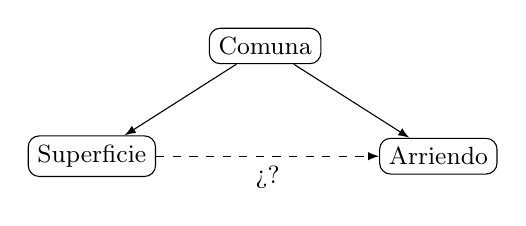
\begin{tikzpicture}[>=latex, every node/.style={font=\small}]
  \node[draw, rounded corners] (C) at (0,1.4) {Comuna};
  \node[draw, rounded corners] (S) at (-2.2,0) {Superficie};
  \node[draw, rounded corners] (A) at (2.2,0) {Arriendo};
  \draw[->] (C) -- (S);
  \draw[->] (C) -- (A);
  \draw[->, dashed] (S) -- (A) node[midway, below] {¿?};
\end{tikzpicture}
\end{center}

A esa tercera variable se le llama una \emph{variable confusora}, y es la pesadilla de cualquiera que quiera sacar conclusiones de los datos. La recta de regresión no distingue entre \enquote{la superficie causa el arriendo} y \enquote{algo más causa a ambos}: ve la misma correlación en los dos casos. Los ejemplos abundan y algunos son ridículos: las ventas de helados y los ahogamientos están correlacionadas, pero no porque el helado ahogue a nadie, sino porque en verano hay más de las dos cosas.

Para hablar de causa de verdad hace falta más que una correlación. O bien un \emph{experimento aleatorizado} ---repartir a la gente al azar entre tratamiento y control, que es justamente por qué la medicina seria lo exige--- o bien un razonamiento causal cuidadoso, con diagramas de flechas que dicen qué causa qué. 

\section{Estadística bayesiana}
\labsec{epi-bayes}

En el capítulo de Bayes aprendimos a actualizar creencias: teníamos una probabilidad a priori, llegaba información, y salía una probabilidad a posteriori. Lo dejamos ahí, como un teorema. Pero sobre esa idea está construida toda una forma alternativa de hacer estadística.

El curso fue basado en el paradigma frecuentista: la probabilidad es una frecuencia a largo plazo, los parámetros de una población son números desconocicos, pero números fijos al fin. La estadística \emph{bayesiana} hace las cosas al revés. Parte de una creencia previa sobre el parámetro expresada como una distribución y la actualiza con los datos para obtener una distribución a posteriori del parámetro. En vez de un intervalo de confianza\sidenote{donde el parámetro no es aleatorio, por lo que la interpretación correcta no es tan fácil como podría parecer}, entrega un \emph{intervalo de credibilidad} del que sí podemos decir lo que nos hubiera gustado: \enquote{hay un \qty{95}{\percent} de probabilidad de que el parámetro esté aquí}. Y recordemos la advertencia del capítulo de pruebas: el valor \(p\) no es la probabilidad de que \(H_0\) sea verdadera. El bayesiano calcula, sin culpa, justo esa probabilidad.

\formal
El motor es siempre el mismo Bayes de antes, ahora con distribuciones: \[\underbrace{p(\theta \mid \text{datos})}_{\text{a posteriori}} \propto \underbrace{p(\text{datos}\mid\theta)}_{\text{verosimilitud}}\;\underbrace{p(\theta)}_{\text{a priori}}.\]
\informal

No es gratis: hay que elegir la distribución a priori, y esa elección es subjetiva. Ahí está la crítica que algunos hacen a esta manera de hacer las cosas, pero por otra parte, el mismo teorema de Bayes nos dice cómo actualizar nuestras probabilidades a medida que vamos aprendiendo más cosas basadas en datos. El debate entre las dos escuelas sigue vivo y es de los más interesantes de toda la disciplina.

\section{Más allá de una recta: regresión múltiple, logística y \emph{machine learning}}
\labsec{epi-ml}

Nuestra regresión usó una sola variable para predecir el arriendo. Pero ya lo dijimos al cerrar ese capítulo: nada nos obliga a quedarnos con una. Con varias variables a la vez —superficie, comuna, antigüedad, número de baños— tenemos \emph{regresión múltiple}, donde la recta se convierte en un plano (o algo de más dimensiones que no se puede dibujar pero sí calcular).

¿Y si lo que queremos predecir no es un número sino un sí o un no? Si un cliente va a pagar el crédito o no, si un correo es spam o no. Ahí entra la \emph{regresión logística}, que en vez de una recta ajusta una curva en forma de S que entrega una probabilidad entre \(0\) y \(1\) —y conecta de vuelta con la variable de Bernoulli, el éxito o fracaso del comienzo del zoológico.

Si empujamos esta idea —ajustar un modelo a los datos para predecir— llegamos al \emph{machine learning}, últimamente bastante de moda. Es la misma historia de la regresión, pero con modelos mucho más flexibles. Esa flexibilidad, como todo, tiene un precio. Si el modelo es demasiado simple, no se ajusta bien a los datos. Si es demasiado flexible, se sobreajusta y toma todo como una señal, hasta lo que es ruido. La forma honesta de saber en qué punto estamos en el eje simpleza-flexibilidad es separar los datos: entrenar el modelo con una parte y evaluarlo con otra que no vio nunca.

\section{Procesos con memoria: cadenas de Markov}
\labsec{epi-markov}

Durante todo el curso insistimos en que la moneda \enquote{no tiene memoria}, y vimos que la distribución exponencial \enquote{olvida} cuánto rato llevamos esperando. ¿Qué pasa cuando \emph{sí} hay memoria? Es decir, ¿qué pasa si las probabilidades futuras dependen del lugar en que estamos?

Una \emph{cadena de Markov} es un sistema que salta entre estados, donde la probabilidad del próximo estado depende del actual —pero sólo del actual, no de toda la historia. El clima sirve de ejemplo de juguete: si hoy hay sol, mañana probablemente siga el sol; si llueve, hay cierta chance de que escampe.

\begin{center}
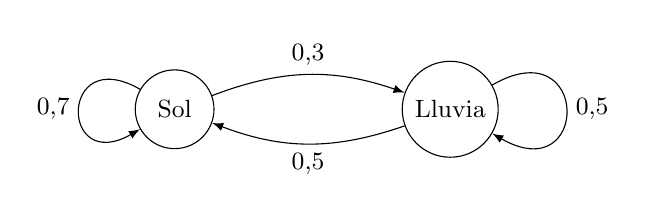
\begin{tikzpicture}[>=latex, every node/.style={font=\small}]
  \node[circle, draw, minimum size=1cm] (S) at (0,0) {Sol};
  \node[circle, draw, minimum size=1cm] (L) at (3.5,0) {Lluvia};
  \draw[->] (S) to[bend left=20] node[above] {\num{0,3}} (L);
  \draw[->] (L) to[bend left=20] node[below] {\num{0,5}} (S);
  \draw[->] (S) to[out=150, in=210, looseness=6] node[left] {\num{0,7}} (S);
  \draw[->] (L) to[out=30, in=-30, looseness=6] node[right] {\num{0,5}} (L);
\end{tikzpicture}
\end{center}

Con esa regla tan simple se modela una variedad sorprendente de cosas: juegos de mesa, el texto que predice la siguiente palabra, el desgaste de una máquina. El ejemplo más famoso es \textsc{PageRank}, el algoritmo con que Google ordenó la web: imagina a alguien navegando al azar de enlace en enlace —una cadena de Markov gigante— y rankea cada página por la fracción del tiempo que ese navegante pasaría en ella. Las cadenas de Markov son la puerta de entrada a los \emph{procesos estocásticos}, donde el azar ya no es un solo experimento sino algo que evoluciona en el tiempo.

\section{Para seguir leyendo (y viendo)}
\labsec{epi-recomendaciones}

Nada de lo anterior se aprende en dos páginas, claro. Acá van recomendaciones para ir en serio. Casi todo está gratis y en línea.

\emph{Para mirar, antes que leer.} \enquote{Seeing Theory}, de la Universidad de Brown (\href{https://seeing-theory.brown.edu/}{{seeing-theory.brown.edu}}), es probabilidad y estadística con visualizaciones interactivas, en el mismo espíritu gráfico de este libro. En video, el canal \href{https://www.youtube.com/@3blue1brown}{\emph{3Blue1Brown}} explica con animaciones hermosas la intuición detrás de Bayes, la binomial y el teorema central del límite; y \href{https://www.youtube.com/@statquest}{\emph{StatQuest}}, de Josh Starmer, desarma casi cualquier tema de estadística con una claridad casi injusta.

\emph{Sobre los gráficos mismos.} Si algo le quedó de este libro es que un buen gráfico vale más que mil cuentas. \enquote{Data Visualization: A Practical Introduction}, de Kieran Healy (gratis en línea, \href{https://socviz.co/}{{socviz.co}}), es un libro entero dedicado a tomarse en serio la visualización: qué hace que un gráfico sea claro, honesto o engañoso. Está muy en sintonía con el espíritu de este texto\sidenote{En realidad, este texto quiere estar en sintonía con el de Healy.}.

\emph{Comparar grupos y estadística clásica.} \enquote{OpenIntro Statistics}, de Diez, Çetinkaya-Rundel y Barr (gratis en \href{https://www.openintro.org/}{{openintro.org}}), cubre con calma las pruebas de dos muestras y el \textsc{anova}.

\emph{Inferencia computacional} (Monte Carlo, bootstrap, permutación). Los libros \enquote{Think Stats} y \enquote{Think Bayes}, de Allen Downey (gratis en \href{https://greenteapress.com/}{{greenteapress.com}}), enseñan estadística programando, justo desde este ángulo. Para ir a la fuente, \enquote{Computer Age Statistical Inference}, de Bradley Efron —el inventor del bootstrap— y Trevor Hastie (PDF gratis), es magnífico.

\emph{Causalidad.} \enquote{The Book of Why}, de Judea Pearl y Dana Mackenzie, es la introducción popular a por qué correlación no es causación. Para algo más técnico pero entretenido, \enquote{Causal Inference: The Mixtape}, de Scott Cunningham (gratis en \href{https://mixtape.scunning.com/}{{mixtape.scunning.com}}).

\emph{Estadística bayesiana.} \enquote{Statistical Rethinking}, de Richard McElreath, es el mejor punto de partida, y el autor subió \href{https://www.youtube.com/playlist?list=PLDcUM9US4XdPz-KxHM4XHt7uUVGWWVSus}{todo su curso en video a YouTube}. Más liviano, el ya mencionado \enquote{Think Bayes}. Y dos videos sueltos que dejan la idea pegada: \href{https://www.youtube.com/watch?v=R13BD8qKeTg}{\enquote{The Bayesian Trap}}, de Veritasium, y \href{https://www.youtube.com/watch?v=HZGCoVF3YvM}{el de Bayes de 3Blue1Brown}.

\emph{Regresión múltiple y machine learning.} \enquote{An Introduction to Statistical Learning}, de James, Witten, Hastie y Tibshirani (gratis en \href{https://www.statlearning.com/}{{statlearning.com}}, con versiones en R y en Python), es el estándar de oro para empezar, y conecta directo con la regresión que acabamos de ver.

\emph{Cadenas de Markov.} La explicación visual interactiva de \href{https://setosa.io/ev/markov-chains/}{{setosa.io}} (\enquote{Markov Chains}) deja la idea clara en cinco minutos de jugar con el mouse.

Hasta aquí llegamos. El jardín de la estadística está lleno de senderos que se bifurcan\sidenote{como un cierto cuento}. Ojalá les parezca un jardín interesante y acogedor, no como el final de \enquote{El Resplandor}. Aunque uno nunca sabe.

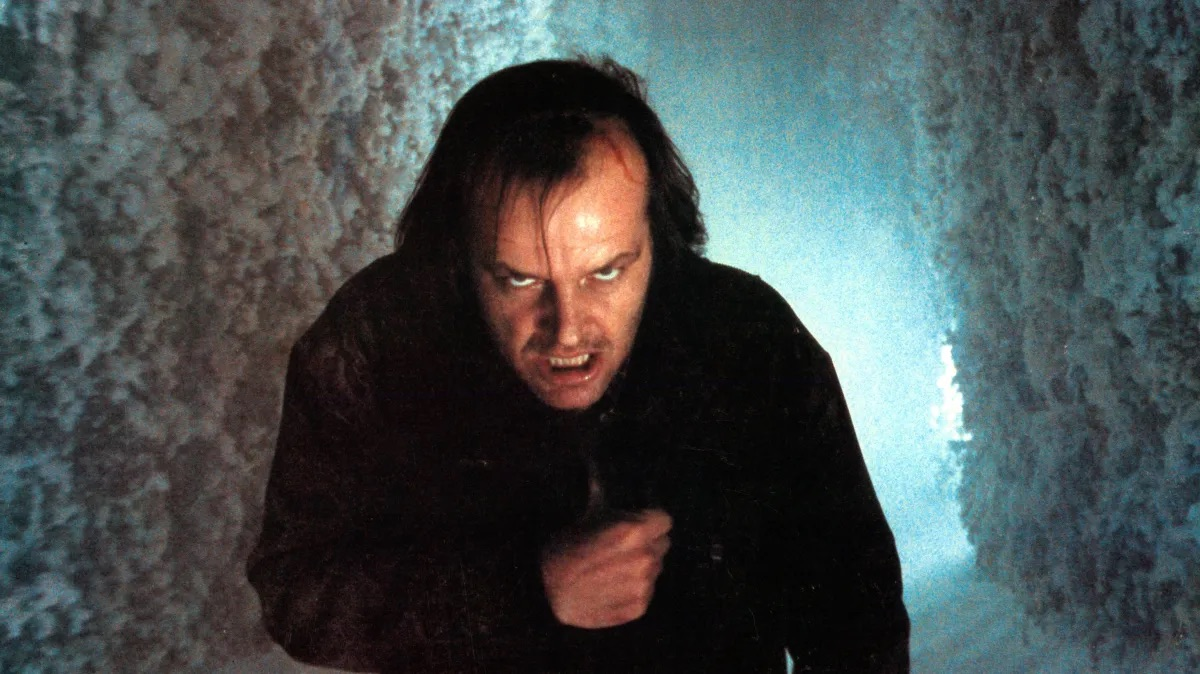
\includegraphics{images/shining.jpg}